\section{Diogenes in a nutshell}

In this section we show the main features of our tools
with the help of a small example.
Suppose we want to implement an online store which 
receives orders from customers,
and relies upon external distributors to retrieve items.

\paragraph{Contracts.}
% A contract describes the intended behaviour of a
% participant involved in a session.
% Session types are terms
% of a process algebra featuring internal/external choice, and
% recursion.
The store has two contracts:
\code{C} to interact with customers, and
\code{D} to interact with distributors.
In \code{C}, the store declares that it will wait for an \atom{order},
and then send either the corresponding \atom{amount} or an \atom{abort} message
(\eg, in case the ordered item is not available).
%
The answer may depend on an external distributor service, 
which waits for a \atom{req}est, and then answers \atom{ok} or \atom{no}.
% 
We write these two contracts as the following 
% first-order 
binary session types~\cite{Honda98esop}:
% 
\begin{lstlisting}[language=coco,basicstyle=\scriptsize\ttfamily]
contract C { order? string . ( amount! int (+) abort! ) }
contract D { req! string . ( ok? + no? ) }
\end{lstlisting}
Receive actions are denoted by the question mark (\code{?}) and grouped
with the symbol \code{+}; similarly, we use the
bang (\code{!}) and the symbol \code{(+)} for send actions. 
We specify the sort of a message 
(\inlineCoco{int}, \inlineCoco{string} or \inlineCoco{unit})
after the action label;
when the sort is omitted, we assume it is \inlineCoco{unit}.

\hidden{The corresponding java contract is
  \begin{mdframed}
    \begin{minted}[
      fontsize=\scriptsize
      % ,linenos
      ]{java}
      ContractDefinition C = def("C").setContract(
      externalSum().add("order", Sort.string(), internalSum()
      .add("amount", Sort.integer())
      .add("abort")));     
      ContractDefinition D = def("D").setContract(
      internalSum().add("req", Sort.string(), externalSum().add("ok").add("no")));
    \end{minted}
  \end{mdframed}
  where \code{def()}, \code{externalSum()}, \code{internalSum()} 
  are static methods of a factory.
}

\paragraph{Specification.}
A naïve \coco specification of our store is the following:
\begin{lstlisting}[
  language=coco,
  basicstyle=\scriptsize\ttfamily,
  numbers=left,
  numbersep=12pt]
specification StoreDishonest {
    tellAndWait x C .
    receive x [
        order? v:string . (
            tellAndWait y D . (
                send y req! v .
                receive y [
                    ok? . send x amount! 100
                    + no? . send x abort!
                    + t . send x abort!]))]
}
\end{lstlisting}

At line \lineno{2}, the store advertises the contract \code{C},
and then waits until a session is established with some customer;
when this happens, the variable \code{x} is bound to the session name.
Then, the store waits to receive an \atom{order}, 
binding it to the variable \code{v} (lines \lineno{3}-\lineno{4}).
At this point the store advertises the contract \code{D}
to establish a session \code{y} with a distributor
(line \lineno{5}); 
after that, it sends a \atom{req}uest (line \lineno{6}) with the value \code{v}.
Finally, the store waits to receive a response \atom{ok} or \atom{no} from the distributor,
and accordingly responds \atom{amount} or \atom{abort} to the customer 
(lines \lineno{7}-\lineno{9}). 
The internal action \inlineCoco{t} models a timeout, 
fired in case no response is received from the distributor (line \lineno{10}).

Our tool correctly detects that the above specification is \emph{dishonest}, by saying:
\begin{lstlisting}[basicstyle=\scriptsize\ttfamily]
result: ("y",$ 0)(
    A[tell "y" D . ask "y" True . (...)] 
    | $ 0["abort" ! unit . 0(+)"amount" ! int . 0])
result: ($ 0,$ 1)(
    A[do $ 0 "abort" ! unit . (0).Sum] 
    | $ 0["abort" ! unit . 0(+)"amount" ! int . 0] 
    | $ 1[ready "no" ? unit . 0])
honesty: false
\end{lstlisting}
The tool output hints the two causes of dishonesty. 
First, if the session \code{y}
is never established (which may happen when no distributor is available), 
the store is stuck at line \lineno{5}
and cannot fulfil the contract \code{C} at session \code{x} (\code{\$0} in the output above).
Second, if the distributor response arrives after the timeout (line \lineno{10}),
the store does not consume the input and 
so it does not respect the contract~\code{D}.

A possible way to fix the above specification is the following:

\vbox{
  \begin{lstlisting}[
    language=coco,
    basicstyle=\scriptsize\ttfamily,
    numbers=left,
    numbersep=12pt]
specification StoreHonest {
    tellAndWait x C .
    receive x [
        order? v:string . (
            tellRetract y D . (
                send y req! v .
                receive y [
                    ok? . send x amount! 100
                    + no? . send x abort!
                    + t . (send x abort! | receive y [ok? + no?])]) 
            : send x abort!)]
}
  \end{lstlisting}
}

The primitive \inlineCoco{tellRetract} at line \lineno{5}
ensures that if the session \code{x} is not established
within a given deadline (immaterial in the specification)
the contract \code{D} is retracted,
and the control passes to line \lineno{11}.
Further, in the timeout branch we have
added a parallel execution of a \inlineCoco{receive}
to consume possible inputs.
Now the tool correctly detects that the revised specification is honest. 

\hidden{The specification does not aim to be completed. On refining the implementation,
  the user must provide suitable timeout values, and 
  the order's amount should be derived in some way.}

\hidden{
  The \cref{fig:outline} shows the outline derived from the above specification.

  \begin{figure}[H]
    \centering
    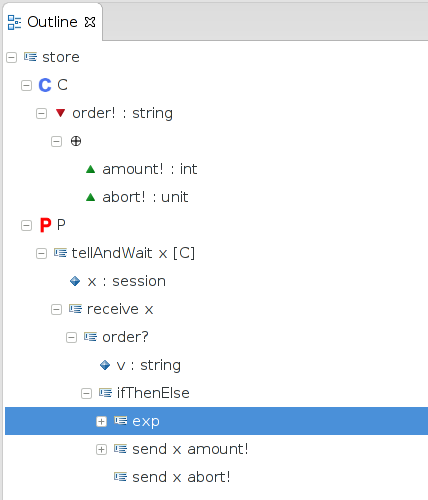
\includegraphics[scale=0.4]{img/outline.png}
    \label{fig:outline}
    \caption{caption}
  \end{figure}
}


\paragraph{Code generation and refinement.}
Diogenes translates \coco specifications into Java skeletons,
using the APIs of the contract-oriented middleware in~\cite{CO2middleware}.
From the honest specification given above,
it generates the following skeleton:
\begin{mdframed}
  \begin{minted}[
    fontsize=\scriptsize
    ,linenos
    ]{java}
public class StoreHonest extends Participant { 
  public void run() {
    Session<TST> x = tellAndWait(C);          // tellAndWait x C
    
    Message msg = x.waitForReceive("order");  // receive c [ order? v:string ]
    String v = msg.getStringValue();
    
    try {
      Session<TST> y = tellAndWait(D, 10000); // tellRetract y D
      y.sendIfAllowed("req", v);
      
      try {                                   // receive y [ok? + no? + t]
        Message msg_1 = y.waitForReceive(10000, "ok", "no");
        switch (msg_1.getLabel()) {                    
          case "ok": x.sendIfAllowed("amount", 100); break;
          case "no": x.sendIfAllowed("abort"); break;                    
        }
      }
      catch (TimeExpiredException e) {        // send x abort! | receive y [ok? + no?] 
        parallel(()->{ x.sendIfAllowed("abort"); });
        parallel(()->{ y.waitForReceive("ok", "no"); });
      }            
    }
    catch(ContractExpiredException e) {
      //contract D retracted
      x.sendIfAllowed("abort");               // : send x abort (line 11)
    } 
  }
}
  \end{minted}
\end{mdframed}

We use Java exceptions to deal with both the \inlineCoco{tellRetract} 
and \inlineCoco{receive} primitives:
the \code{ContractExpiredException} is thrown by line \lineno{9} if the session \code{y}
is not established within ten seconds, while the \code{TimeExpiredException}
is thrown by line \lineno{13} if a message is not received within (again) ten seconds.
The \code{parallel} method at lines \lineno{20}-\lineno{21} starts a new 
thread that will execute the passed \code{Runnable} instance.
%
The timeout values, as well as the order amount at line \lineno{15}, are just placeholders;
% hardcoded in the skeleton.
in an actual implementation of the store service, we may want to delegate the computation the \code{amount} to a separated method, \eg:
\begin{mdframed}
  \begin{minted}[
    fontsize=\scriptsize
    % ,linenos
    ]{java}
    public int getOrderAmount(String order) throws MyException {...}
  \end{minted}
\end{mdframed}
and change the number \code{100} at line \lineno{15} with \code{getOrderAmount(v)}.
The method could read the order amount from a file or a database,
and suppose that each possible exception
is caught and hidden behind \code{MyException}. 
The failure of this method can be considered non-deterministic,
so we need to ``instruct'' our verification tool
in order to consider all the possible ways the method can terminate.
% 
To this purpose, we provide the annotation \code{@SkipMethod(value="<value>")}, that
is interpreted by the checker as follows:
\begin{inlinelist}[noitemsep,topsep=0pt]
\item ignore what the method really does (it imposes that an annotated 
    method does not perform any action directed to the middleware);
\item consider \code{<value>} as the returning value on success;
\item consider the declared exceptions as possible exit points on failure.
\end{inlinelist}
%
Diogenes can symbolically consider both the case of a normal 
termination of the method
%(returning the value specified in the annotation, if provided),
and all the possible exceptional terminations.

\paragraph{Verification.}
Diogenes can verify the honesty of Java programs 
by invoking the static method
\code{HonestyChecker.isHonest(StoreHonest.class)},
which returns one of the following values:
\begin{itemize}[noitemsep,topsep=0pt]
\item \code{HONEST}: the tool has extracted a \coco specification and verified its honesty;
\item \code{DISHONEST}: as above, but the \coco specification is dishonest;
\item \code{UNKNOWN}: the tool has been unable to extract a \coco specification,
  \eg because of unhandled exceptions within the class under test.
\end{itemize}

\noindent
For our refined store, the Java honesty checker returns \code{UNKNOWN} and outputs:
\begin{mdframed}
  \begin{minted}[
    fontsize=\scriptsize
    % ,linenos
    ]{java}
error details: MyException: 
    This exception is thrown by the honesty checker. Please catch it!
    at it.unica.co2.store.Store$Phonest.getOrderAmount(Store.java:166)
    at it.unica.co2.store.Store$Phonest.run(Store.java:129)
    at it.unica.co2.honesty.HonestyChecker.runProcess(HonestyChecker.java:182)
  \end{minted}
\end{mdframed}
This means that if the method \code{getOrderAmount} fails
the program will be terminated abruptly, and so the store may violate the contract.
We can recover honesty by catching \code{MyException} with \code{x.sendIfAllowed("abort")}.
With this modification, the Java honesty checker correctly outputs \code{HONEST}.

